\chapter{Conexión con openssl s\_client}
\section{Enunciado}
7. Conexión desde \texttt{openssl s\_client} a \texttt{www.ejemplo.com:443} y comparación de las primeras líneas de la conexión con la conexión a \texttt{www.ulpgc.es:443}; asegurarse de que no hay problema en la identificación del servidor y los certificados que presenta.
\section{Resolución}
Se utiliza el comando \texttt{openssl s\_client} para conectarse al servidor y verificar la información del certificado presentado por el servidor. La orden es la siguiente:
\begin{lstlisting}[language=bash]
openssl s_client -connect www.ejemplo.com:443
\end{lstlisting}
\begin{figure}
    \centering     % Centra la imagen (buena práctica)

    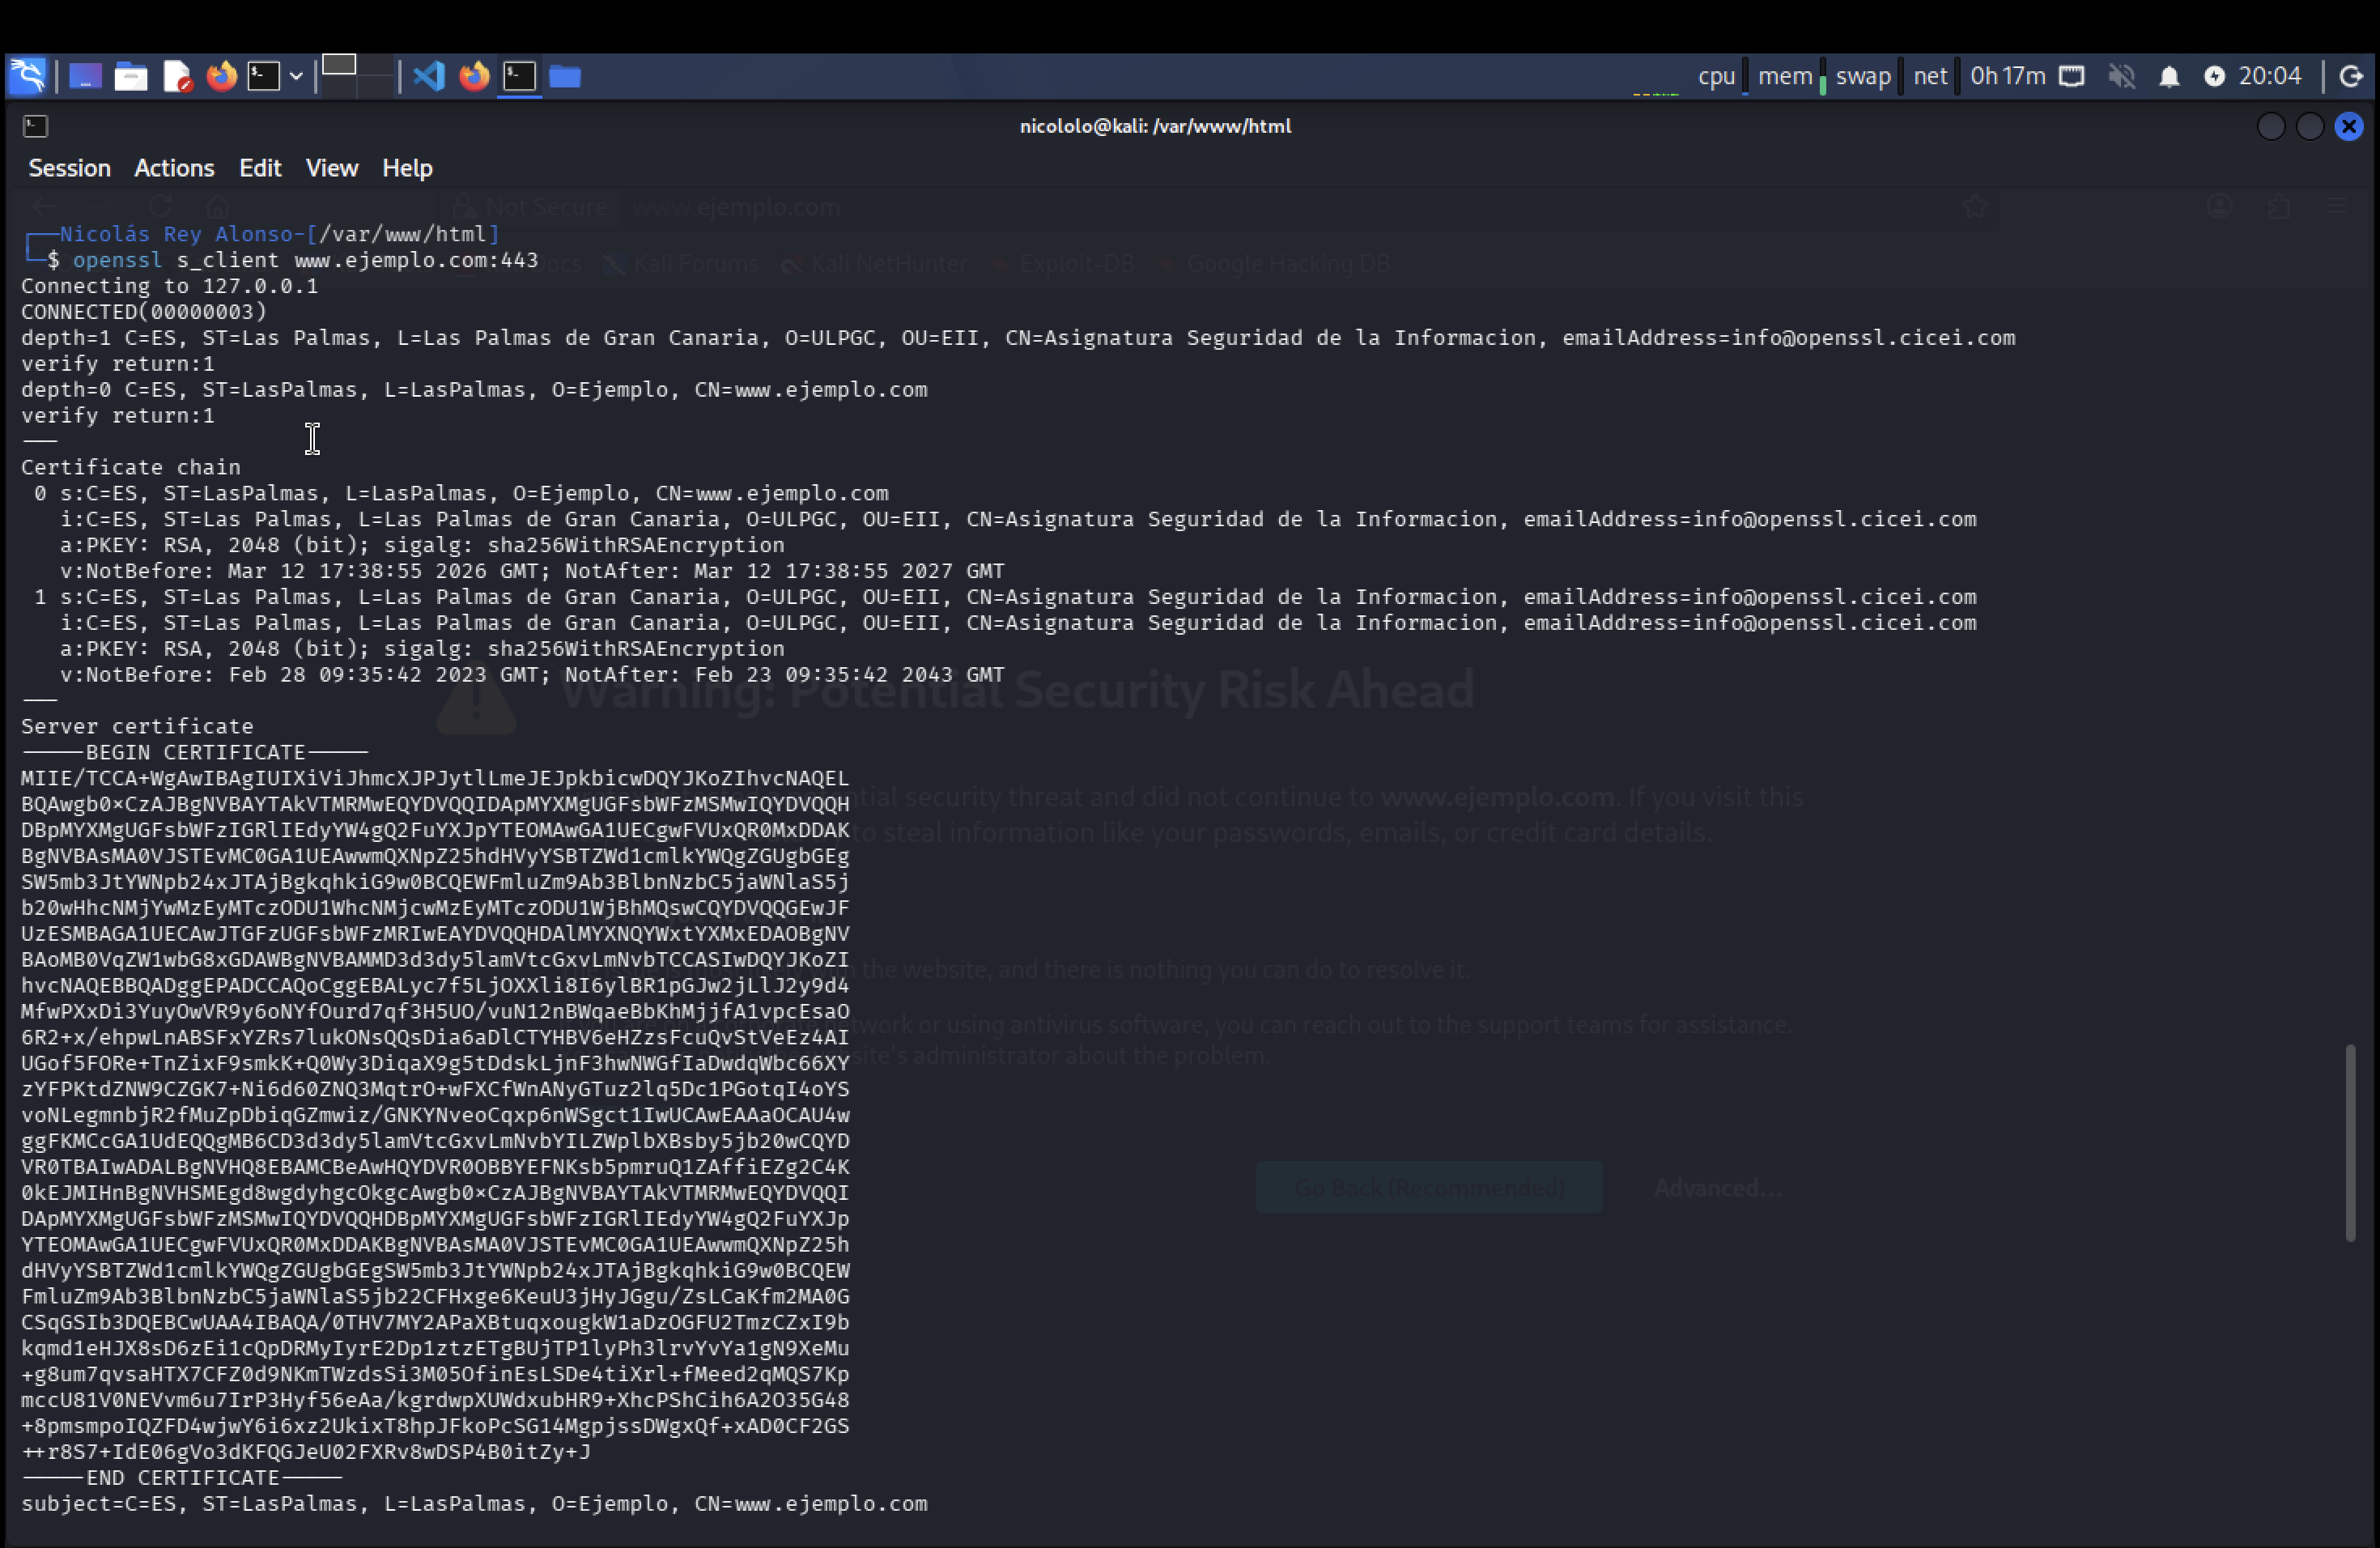
\includegraphics[width=0.8\textwidth]{Imagenes/16.png}
    
    \caption{Conexión con openssl s\_client a www.ejemplo.com:443.} 
    
    \label{fig:imagen_16} % Etiqueta para poder referenciarla más tarde
\end{figure}
Se compara con la conexión a \texttt{www.ulpgc.es:443} para verificar. 
Así nos aseguramos de que no hay un problema de identificación del servidor y los 
certificados que presenta.
\begin{lstlisting}[language=bash]
openssl s_client -connect www.ulpgc.es:443
\end{lstlisting}
\begin{figure}
    \centering     % Centra la imagen (buena práctica)

    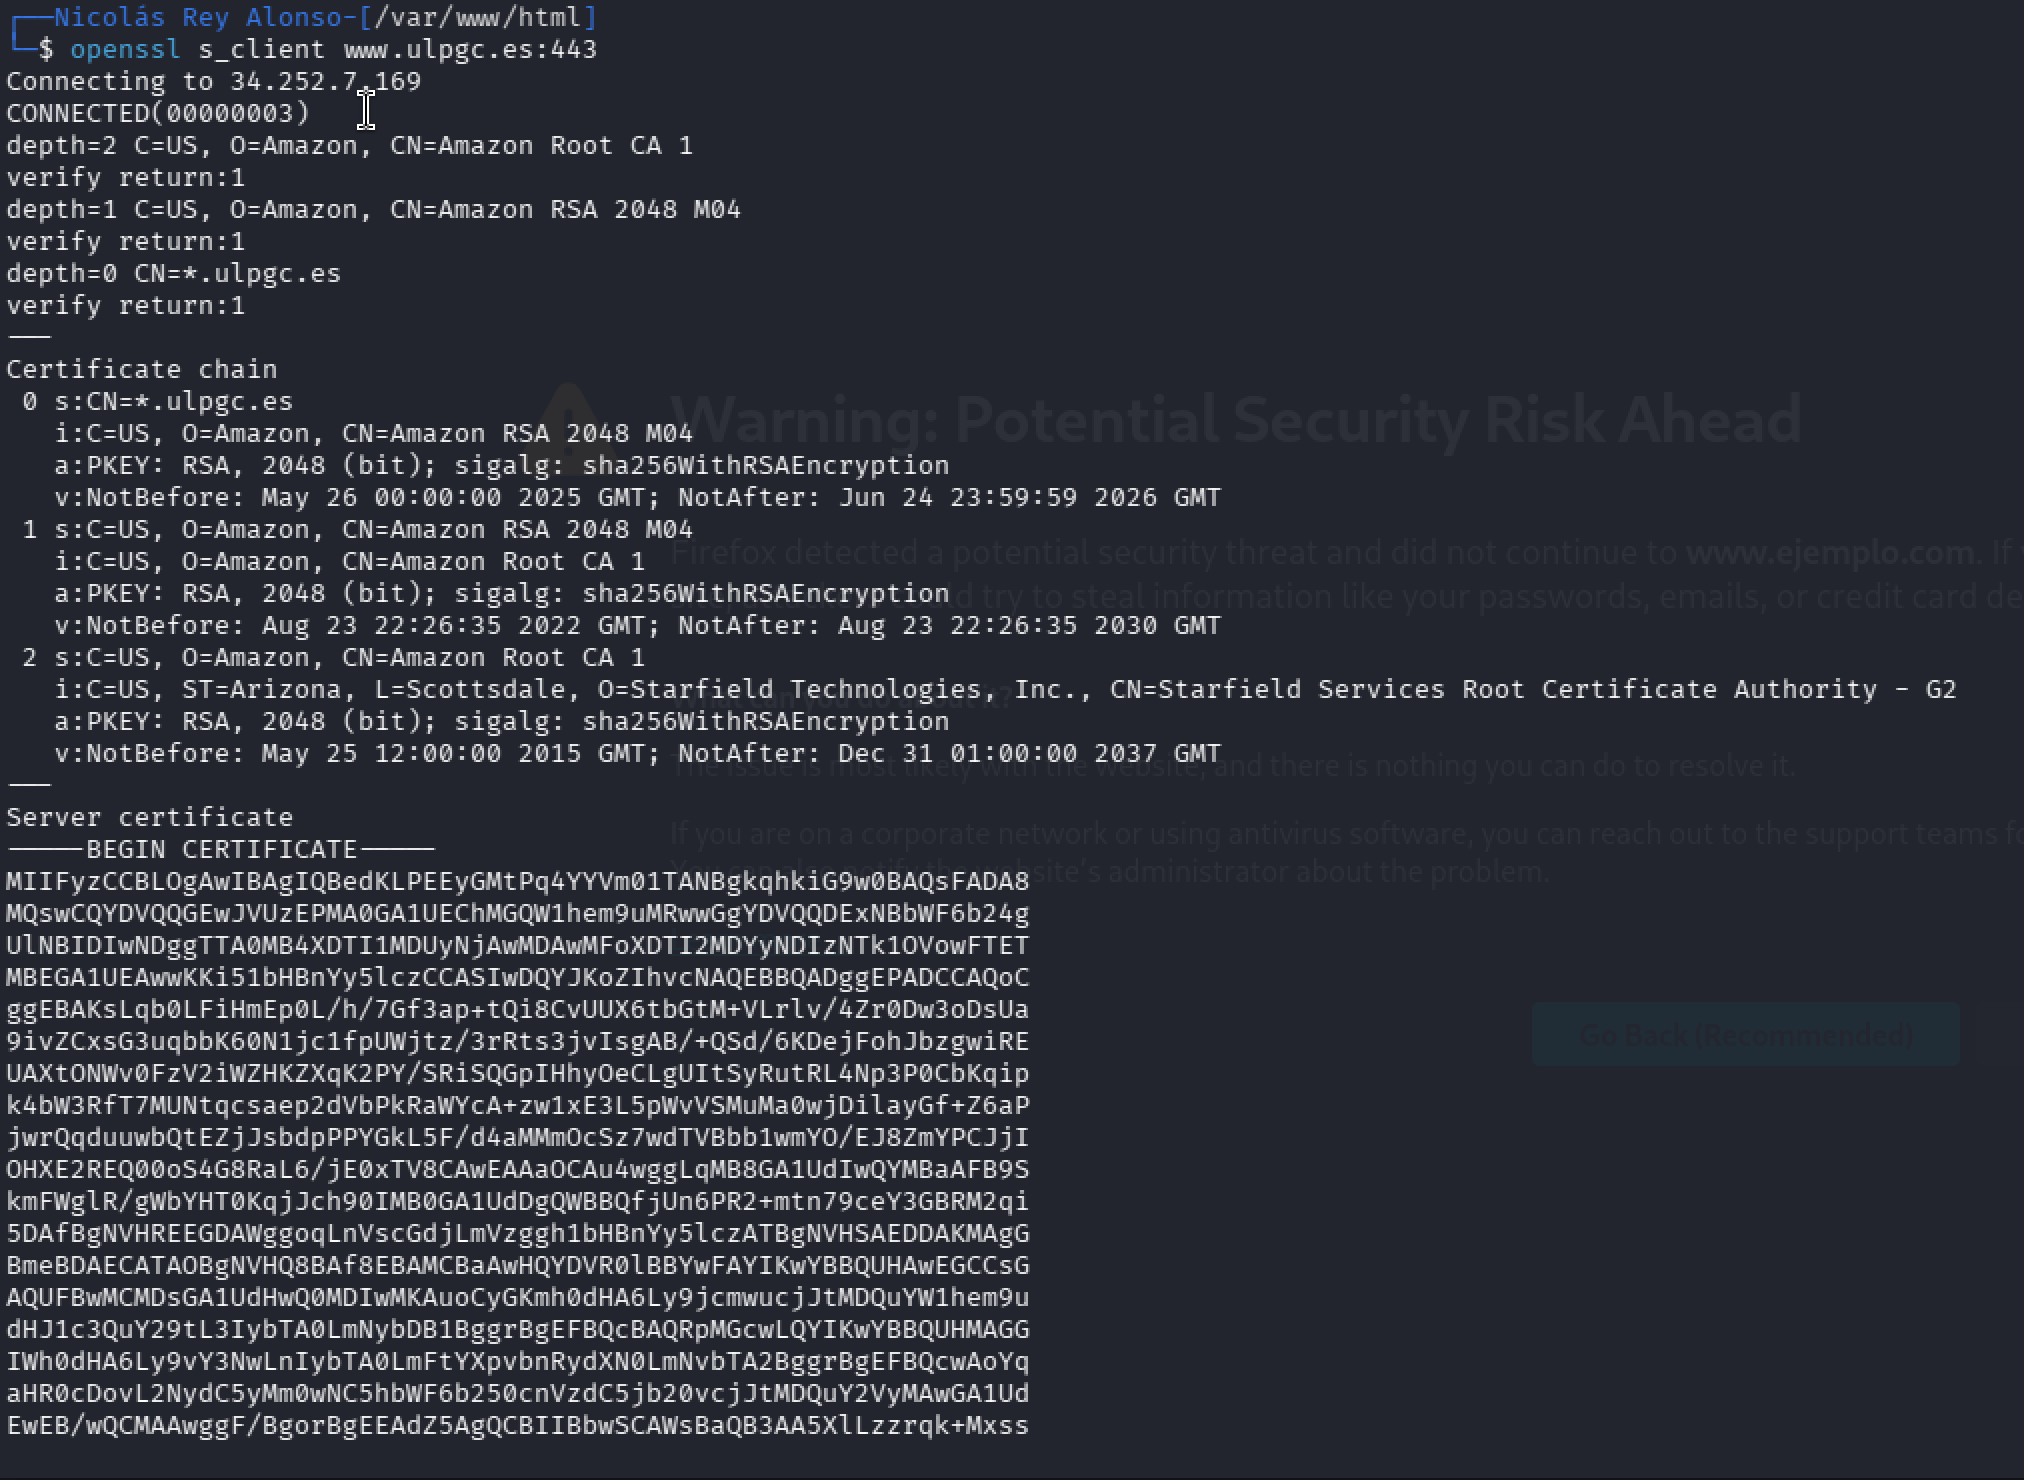
\includegraphics[width=0.8\textwidth]{Imagenes/17.png}
    
    \caption{Conexión con openssl s\_client a www.ulpgc.es:443.} 
    
    \label{fig:imagen_17} % Etiqueta para poder referenciarla más tarde
\end{figure}
